\section{Auswertung}
\label{sec:Auswertung}
Da eine lineare Abhängigkeit zwischen der Spannung $U_\text{k}$ und der Stromstärke $I$ nach Formel ??? besteht,
wird im Folgenden eine lineare Regression sowie die Bestimmung der zugehörigen Fehler mit
IPython 5.1.0 mittels Scipy 0.18.1 durchgeführt.
Die Parameter der Ausgleichsgeraden
\begin{equation}
\label{eqn:ausgleichsgrade}
y=a \cdot x +b .
\end{equation}
werden dabei bestimmt über

\begin{equation*}
\label{eqn:ausgleichsgrade_a}
a= \frac{ \overline{xy}- \overline{x} \cdot \overline{y}}{\overline{x^2}-\overline{x}^2} .
\end{equation*}

\begin{equation*}
\label{eqn:ausgleichsgrade_b}
b= \frac{ \overline{x^2} \overline{y}- \overline{x} \cdot \overline{xy}}{\overline{x^2}-\overline{x}^2} .
\end{equation*}

Die direkt an der Monozelle abgegriffene Leerlaufspannung $U_\text{0}$ ergibt sich zu $1.5 \,\si{\ohm}$.
Der Fehler des Voltmeters beträgt nach Herstellerangaben im verwendeten Messbereich $1.5\%$.
Damit ergibt sich $U_\text{0}=(1.5 \pm 0.0225) \,\si{\ohm}$.
Der Innenwiderstand des Voltmeters ist nach Herstellerangaben $R_\text{V}\approx 10 \cdot 10^6 \,\si{\ohm}$.

Der Innenwiderstand $R_\text{i}$ und die Leerlaufspannung $U_\text{0}$ der Monozelle ergeben sich mit
Linearer Regression nach \eqref{eqn:ausgleichsgrade} unter Verwendung von Formel ???.
Dazu werden die in Tabelle \ref{tab:mono} gelisteten $U_\text{k}$ gegen $I$ aufgetragen. Der zugehörige Plot ist in Abbildung \ref{fig:plot_a} zu sehen.

\begin{equation*}
  -a= R_\text{i}=(15.5\pm0.3)\,\si{\ohm}
\end{equation*}
\begin{equation*}
  b =U_\text{0}=(1501.4\pm13.9)\,\si{\milli\volt}
\end{equation*}


\begin{table}
  \centering
  \caption{Messdaten für die Klemmenspannung in Abhängigkeit des Strom bei der Monozelle}
  \label{tab:mono}

\begin{tabular}{cc}
  \toprule
$U_\text{k}$/$\,\si{\milli\volt}$ & $I$/$\,\si{\milli\ampere}$\\
\midrule
69.0 & 91.0 \\
342.0 & 74.0 \\
550.0 & 61.0 \\
700.0 & 52.0 \\
825.0 & 45.0 \\
910.0 & 40.0 \\
965.0 & 37.0 \\
980.0 & 35.0 \\
990.0 & 32.0 \\
1026.0 & 30.0 \\
1056.0 & 28.0 \\
1083.0 & 26.0 \\
1110.0 & 24.0 \\
1116.0 & 23.0 \\
\bottomrule
\label{tab:labbadia}
\end{tabular}
\end{table}
\begin{figure}
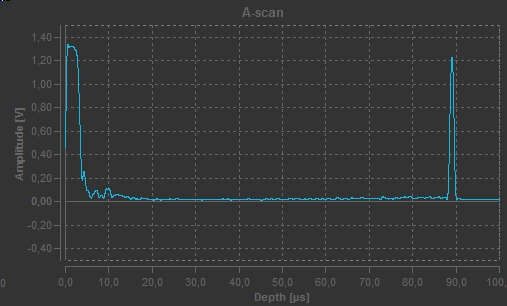
\includegraphics{Bilder/a.pdf}
\caption{Linearer Fit zur Monozelle ohne Gegenspannung}
\label{fig:plot_a}
\end{figure}


%monozelle belastet
Die Messung der Leerlaufspannung $U_\text{0}$ und des Innenwiderstandes $R_i$ der Monozelle wird mit den Daten der Messreihe mit Gegenspannung wiederholt. Hierbei ist die Stromrichtung nun umgekehrt, sodass sich das Vorzeichen in Gleichung ??? umkehrt.
Mit den Messdaten aus Tabelle \ref{tab:monozelle_belastet} ergibt sich der zugehörige Plot in \ref{fig:plot_monozellebelastet} mit \eqref{eqn:ausgleichsgrade}. Damit erhält man:

\begin{equation*}
  a= R_\text{i}=(17.3\pm 0.5)\,\si{\ohm}
\end{equation*}
\begin{equation*}
  b =U_\text{0}=(1626.3\pm 26.1)\,\si{\milli\volt}\,.
\end{equation*}
\begin{table}
  \centering
  \caption{Messdaten für die Klemmenspannung in Abhängigkeit des Strom bei der Monozelle mit Gegenspannung}
  \label{tab:monozelle_belastet}
\begin{tabular}{cc}
  \toprule
$U_\text{k}$/$\,\si{\milli\volt}$ & $I$/$\,\si{\milli\ampere}$\\
\midrule
3400.0 & 99.0 \\
3100.0 & 92.0 \\
2850.0 & 68.0 \\
2700.0 & 58.0 \\
2460.0 & 49.0 \\
2340.0 & 42.0 \\
2250.0 & 37.0 \\
2160.0 & 33.0 \\
2100.0 & 29.0 \\
2070.0 & 26.0 \\
2040.0 & 24.0 \\
2010.0 & 21.0 \\
1980.0 & 20.0 \\
1970.0 & 19.0 \\
\bottomrule
\end{tabular}
\end{table}
\begin{figure}
\includegraphics{Bilder/c.pdf}
\caption{Linearer Fit zur Monozelle mit Gegenspannung}
\label{fig:plot_monozellebelastet}
\end{figure}

Die Berechnung der Ausgleichsgeraden für die Rechteck-und Sinusspannungsquelle ergeben sich analog zu den Berechnungen bei der Monozelle.


%rechteckspannung
Die Leerlaufspannung $U_\text{0}$ und den Innenwiderstand $R_\text{i}$ der Rechteckspannung ergeben sich mit den Daten aus Tabelle \ref{tab:reckteck} und der Ausgleichsgraden in Plot \ref{fig:plot_rechteck} zu:
\begin{equation*}
  -a= R_\text{i}=(69.1\pm0.7)\,\si{\ohm}
\end{equation*}
\begin{equation*}
  b =U_\text{0}=(477.8\pm1.4)\,\si{\milli\volt}
\end{equation*}
Die Leerlaufspannung $U_\text{0}$ und der Innenwiderstand $R_\text{i}$ der Sinusspannung ergeben sich mit den Daten aus Tabelle \ref{tab:sinus} und der Ausgleichsgraden in Plot \ref{fig:plot_sinus} zu:
%sinusspannung
\begin{equation*}
  -a= R_\text{i}=(657.0± 5.0)\,\si{\ohm}
\end{equation*}
\begin{equation*}
  b =U_\text{0}=(1567.4\pm3.6)\,\si{\milli\volt}
\end{equation*}

\begin{table}
  \centering
  \caption{Messdaten für die Klemmenspannung in Abhängigkeit des Strom bei der Rechteckspannungsquelle}
  \label{tab:reckteck}
\begin{tabular}{cc}
  \toprule
$U_\text{k}$/$\,\si{\milli\volt}$ & $I$/$\,\si{\milli\ampere}$\\
\midrule
165.0 & 4.5 \\
195.0 & 4.1 \\
245.0 & 3.4 \\
295.0 & 2.6 \\
325.0 & 2.2 \\
345.0 & 1.9 \\
365.0 & 1.7 \\
380.0 & 1.4 \\
395.0 & 1.2 \\
405.0 & 1.1 \\
415.0 & 1.0 \\
420.0 & 0.8 \\
425.0 & 0.7 \\
430.0 & 0.68 \\
430.0 & 0.67 \\
\bottomrule
\end{tabular}
\end{table}
\begin{figure}
\includegraphics{Bilder/d.pdf}
\caption{Linearer Fit zur Rechteckspannung}
\label{fig:plot_rechteck}
\end{figure}

\begin{table}
  \centering
  \caption{Messdaten für die Klemmenspannung in Abhängigkeit des Strom bei der Sinusspannungsquelle}
  \label{tab:sinus}

\begin{tabular}{cc}
  \toprule
$U_\text{k}$/$\,\si{\milli\volt}$ & $I$/$\,\si{\milli\ampere}$\\
\midrule
510.0 & 1.62 \\
675.0 & 1.35 \\
960.0 & 0.93 \\
1125.0 & 0.66 \\
1230.0 & 0.51 \\
1320.0 & 0.36 \\
1395.0 & 0.27 \\
1425.0 & 0.21 \\
1455.0 & 0.18 \\
1485.0 & 0.15 \\
1491.0 & 0.12 \\
1500.0 & 0.09 \\
\bottomrule
\end{tabular}
\end{table}
\begin{figure}
\includegraphics{Bilder/e.pdf}
\caption{Linearer Fit zur Sinusspannung}
\label{fig:plot_sinus}
\end{figure}
Bisher wurde für die Berechnungen vereinfachend angenommen worden,
dass der Term $-IR_\text{i}$ in Gleichung \eqref{eqn:klemmu} vernachlässigt werden kann. Im realen Fall ist allerdings der Innenwiderstand $R_\text{V}$ des Voltmeters nicht unendlich groß.
Somit ergibt sich mit dem Ohmschen Gesetz ein systematischer Fehler bei der direkten Leerlaufspannungsmessung:
\begin{equation*}
  U_\text{k}=I\cdot R_\text{a} \leftrightarrow I=\frac{U_\text{k}}{R_\text{V}}\, ;
\end{equation*}
da im vorliegenden Fall, wie in Abbildung \ref{fig:abbildung1} zu sehen, $R_\text{a}=R_\text{V}$ gilt, ergibt sich mit Gleichung \eqref{eqn:klemmu}
\begin{equation*}
U_\text{0}=U_\text{k}+\frac{R_\text{i}}{R_\text{V}}\cdot U_\text{k}\, .
\end{equation*}
Damit ergibt sich der Fehler
\begin{equation*}
  \Delta  U_\text{0}=\frac{R_\text{i}}{R_\text{V}} \, .
\end{equation*}
Mit $R_\text{V}=10 \cdot 10^6 \,\si{\ohm}$ und $R_\text{i}=(15.5\pm0.3)\,\si{\ohm}$ ergibt sich für die Monozelle
\begin{equation*}
\Delta U_\text{0}= (1.55 \pm 0.03)\cdot 10^{-6}\, \si{\ohm}
\end{equation*}
Da der direkt gemessene Wert $U_\text{0}=(1.5 \pm 0.0225)\, \si{\ohm}$ betrug, ergibt sich ein Fehler von $\frac{\Delta U_\text{0}}{U_\text{0}}=(1.033\pm0.025)\cdot 10^{-6} \%$.
Dieser systematische Fehler ist sehr gering und wird daher im Weiteren vernachlässigt.

Des Weiteren würde man einen systematischen Fehler machen, wenn man in Abbildung \ref{fig:abbildung2} das Voltmeter hinter das Amperemeter - also an den Punkt H legt.
Dies liegt daran, dass durch den Innenwiderstand des Amperemeters ein weiterer Spannungsabfall zu berücksichtigen ist. Daher würde man nicht die zuvor definierte Klemmenspannung $U_{\text{K}}$ messen.

Die abgegebende Leistung $N$ in Abhängigkeit vom Belastungswiderstand $R_{\text{a}}$ ist in Abbildung \ref{fig:aufe} dargestellt. 
Hierzu wird die Theoriekurve mit der rechten Seite der Formel \eqref{eqn:leistung} bestimmt.
Die Werte $N$ für die abgegebende Leistung, die sich aus den Messdaten $U_{\text{K}}$ und $I$ aus Tabelle \ref{tab:labbadia} ergeben, werden allerdings mit der linken Seite der Formel \eqref{eqn:leistung} berechnet.
\begin{figure}
\includegraphics{Bilder/leistung.pdf}
\caption{Abgegebende Leistung in Abhängigkeit vom Belastungswiderstand}
\label{fig:aufe}
\end{figure}

Die Abweichungen der einzelnen Messpunkte zur Theoriekurve $N(R_{\text{a}})$ lassen sich nicht auf einen systematischen Fehler zurückführen.
Zuerst lässt sich anmerken, dass die größte Abweichung von der Theoriekurve bei $R_{\text{a}} \approx \SI{26,1}{\ohm}$ mit ungefähr $5,3 \, \%$ gering ausfällt. Daher herrscht eine geringe Diskrepanz zwischen den Messwerten und der Theoriekurve.
Des Weiteren liegen die Messpunkte sowohl über- als auch unterhalb der Theoriekurve, was ein weiteres Indiz für ausschlaggebende zufällige Fehler ist.
Der systematische Fehler beispielsweise bei der direkten Messung der Leerlaufspannung $U_0$ ist - wie vorher angenommen - vernachlässigbar in Relation zu den zufälligen Fehlern bei diesen Messungen.

Das Maximum der Leistung liegt bei $R_{\text{a}} \approx R_{\text{i}} = (15,5 \pm 0,3) \, \si{\ohm}$ - was auch nach der Theorie zu erwarten war.

